\documentclass[12pt, a4paper, openany]{report}

\def\VersionRapport{1.0}

\usepackage[utf8]{inputenc} % un package
\usepackage[T1]{fontenc}      % un second package
\usepackage[francais]{babel}  % un troisième package
\usepackage{layout}
\usepackage[top=2.7cm, bottom=2.5cm, left=3.5cm, right=3cm]{geometry}
\usepackage{setspace}

\frenchbsetup{StandardLists=true} % à inclure si on utilise \usepackage[french]{babel}
%\usepackage{enumitem}
\usepackage[shortlabels]{enumitem}
\usepackage{amssymb}

\usepackage{color}
\usepackage{listings}
\definecolor{dkgreen}{rgb}{0,0.6,0}
\definecolor{gray}{rgb}{0.5,0.5,0.5}
\definecolor{mauve}{rgb}{0.58,0,0.82}

\lstset{frame=tb,
  language=Matlab,
  aboveskip=3mm,
  belowskip=3mm,
  showstringspaces=false,
  columns=flexible,
  basicstyle={\small\ttfamily},
  keywordstyle=\color{blue},
  commentstyle=\color{dkgreen},
  stringstyle=\color{mauve},
  breaklines=true,
  breakatwhitespace=true,
  tabsize=3,
  breaklines=true,
  morekeywords={matlab2tikz},
  morekeywords=[2]{1}, 
  keywordstyle=[2]{\color{black}},
  identifierstyle=\color{black},
  numbers=left,
  numberstyle={\tiny \color{black}},
  numbersep=9pt, 
  emph=[1]{for,end,break},
  emphstyle=[1]\color{red}
}



\usepackage{multirow} % pour les tableaux
\usepackage[table]{xcolor} % pour les tableaux

\usepackage{verbatim}
\usepackage{moreverb}
\usepackage{url}
\usepackage{pst-all}
\usepackage{eso-pic,graphicx}
\usepackage{caption} 
\usepackage[colorlinks=true,urlcolor=blue,linkcolor=red]{hyperref}
\usepackage{array}
\usepackage[toc,page]{appendix}
\usepackage[off]{auto-pst-pdf}
\usepackage{hyperref} % pour le sommaire table des matières
\AddThinSpaceBeforeFootnotes % à insérer si on utilise \usepackage[french]{babel}
\FrenchFootnotes % à insérer si on utilise \usepackage[french]{babel}
\usepackage{fancyhdr}
\pagestyle{headings}
\usepackage{pifont}  %pour les puces
\usepackage{amsmath} %pour les puces

\usepackage{verbatim} % pour le code en annexe 

%%%%%%%colones 
\newcolumntype{R}[1]{>{\raggedleft\arraybackslash }b{#1}}
\newcolumntype{L}[1]{>{\raggedright\arraybackslash }b{#1}}
\newcolumntype{C}[1]{>{\centering\arraybackslash }b{#1}}
%%%%%%% 

\renewcommand{\appendixpagename}{Annexes}
\renewcommand{\appendixtocname}{Annexes}

\title{Theme: Compte Rendu Système Linéaire à Temps Continu 1}
\author{REBOUT \bsc{Mehenna}}
\author{BOUYOUCEF \bsc{Farid}}
\date{2018-2019}



%new
\newcommand{\HRule}{\rule{\linewidth}{0.5mm}}


\begin{document}

%\selectlanguage{francais}
\pagenumbering{arabic} 

\makeatletter
  \begin{titlepage}
  

  \begin{sffamily}
   \begin{center}

    % Upper part of the page. The '~' is needed because \\
    % only works if a paragraph has started.
    
\includegraphics[scale=0.5]{Logo_UT3.jpg}~\\[1.5cm]

    \textsc{\LARGE Master 1 EEA ISTR/RODECO  }\\[2cm]

    \textsc{\Large Compte Rendu  Système Linéaire à Temps Continu 1}\\[1.5cm]

    % Title
    \HRule \\[0.4cm] % saut de ligne
    { \huge \bfseries TP 3 BACS D’EAU\\[0.4cm] }

    \HRule \\[1cm]   % sous de ligne 
    
\includegraphics[scale=0.1]{logomaster.jpg}
    \\[1cm]

    % Author and supervisor
    \begin{minipage}{0.4\textwidth}
      \begin{flushleft} \large
         \textsc{\emph {Réalisés par:} \\REBOUT Mehenna}\\
         \textsc{BOUYOUCEF Farid}   
          \newline
          Promotion 2018-2019 \\
      \end{flushleft}
    \end{minipage}
    \begin{minipage}{0.4\textwidth}
      \begin{flushright} \large
        \emph{Tuteur :}  \textsc{M DUROLA}\\
        \emph{Responsable de la Formation:} \textsc{M GOUAISBAUT}
      \end{flushright}
    \end{minipage}

    \vfill

    % Bottom of the page
    {\large Octobre 2018}

  \end{center}
  \end{sffamily}      
          
  \end{titlepage}
  
\makeatother




   
%*********************** somaire **************
\renewcommand{\contentsname}{Sommaire}
\tableofcontents
%*********************** listes des figures **************
\listoffigures
%*********************** listes des tableaux **************
\listoftables
 
 
 
 %*********************** INTRODUCTION **************
\chapter*{Introduction}Dans ce TP on va réaliser un asservissement de position ,on va utiliser pour cette manipulation la platine voir   la Figure 1.1.
\addcontentsline{toc}{chapter}{Introduction}



Les valeurs numériques des coefficients connus sont:\\

 $K_e=10(V.tr^-1)$	 \hfill		$K_s=10(V.tr^-1)$	\hfill		$Kg=0.105(V.s.tr^-1)$ 
 %Farid
\chapter{ L'objet du TP }
\addcontentsline{toc}{chapter}{L'objet du TP} 
 
  \section{Objet Du TP}
      Le but de cette manipulation est de réaliser un asservissement de niveau par retour de sortie. En effet, le vecteur d’état du procédé hydraulique n’est pas entièrement accessible par la mesure. On se propose ainsi de mettre en œuvre l’estimation de l’état par un observateur.
  
  
 %Farid
\chapter{Présentation  Du Système }
\addcontentsline{toc}{chapter}{Présentation  Du Système }

 \section{Le Procède}

      Le procédé est le même que celui qui a été utilisé dans le TP du module I4 intitulé "Modélisation, analyse et com-mande d’une distribution hydraulique à trois bacs d’eau". Nous redonnons ici les caractéristiques essentielles de la manipulation.
      
\begin{center}
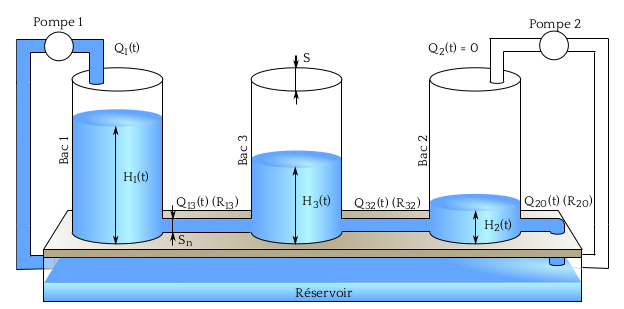
\includegraphics[scale=0.5]{fig1.png}
\captionof{figure}{\textit{ Procédé trois bacs.\cite{ref1}}}
\label{fig1} 
\end{center}

      Le système représenté sur la Figure 2.1 est composé de trois bacs cylindriques en plexiglas de section S. Ces trois bacs sont disposés en série (de gauche à droite, on trouve les bacs 1, 3 et 2) et sont reliés par des tuyaux d’écoulement de section S n .
      
      Le dernier bac 2 se vide par un cylindre, également de section S n , dans le réservoir situé sous les bacs. Deux pompes de débit Q 1 (t) et Q 2 (t) permettent de remplir respectivement les bacs 1 et 2 avec l’eau récupérée dans le réservoir, le système fonctionnant en circuit fermé.

      Les valeurs données par le constructeur sont S = 0, 0154m 2 et S n = 5.10 –5 m 2 .
      Les pompes obéissent à la relation V qi (t) = k · Q i (t) + b, i = 1, 2, avec k = 1, 6.10 5 et b = –9, 2592; où V qi et Q i (t) représentent respectivement la tension appliquée à la pompe i et le débit correspondant.
      Les pompes sont alimentées par une tension comprise entre [–10V, 10V]. Ainsi le débit maximal, Q max
délivrée par une pompe est 12.10 –5 m 3 /s lorsque la tension appliquée est de +10V. Les capteurs de niveau d’eau sont supposés linéaires autour du point de fonctionnement. Leur caractéristique est modélisé par l’équation H i (t) = k i · V h i (t) + b i , où H i est exprimé en mètres.\cite{ref1}


 \section{Le Modèle Linéarisé }
 
      Nous considérons le procédé actionné par la seule pompe numéro 1. Son débit Q 1 est compris entre [0, Q max ] suivant sa tension d’alimentation; le débit Q 2 (t) délivré par la pompe 2 sera nul tout au long de la manipulation. Ainsi, les différentes hauteurs H 1 (t), H 3 (t) et H 3 (t) respectent par conséquent la condition H{1}(t)$\geq$H{3}(t)$\geq$H{2}(t).\\ 
      La seule mesure disponible lors de cette manipulation est la mesure de la hauteur d’eau H 1 .\\
      
      Le travail sera réalisé sur un modèle aux faibles variations autour d’un point d’équilibre H 0 et d’un débit Q 10 à ce point d’équilibre de telle sorte que:

\begin{equation}
\left\{\begin{matrix}
Q1(t)=q1(t) +Q10\\
H{1}(t)=h{1}(t) +H{10}\\
H{3}(t)=h{3}(t) +H{30}\\
H{2}(t)=h{2}(t) +H{20}\\
\end{matrix}\right.
\end{equation} 


$H{0}$=$\begin{bmatrix}
H{10}\\
H{20}\\
H{30}\\
\end{bmatrix}$
\quad=\quad
$\begin{bmatrix}
0.27474\\
0.0299\\
0.1368\\
\end{bmatrix}$\\\\

$Q{10}$=$3.5*10^{-5}$\\

Le modèle D’état est\\


$\dot{h}(t)$=$\begin{bmatrix}
-0.0092 & 0.0092 & 0 \\
0.0092 & -0.0198 & 0.0106\\
0 & 0.0106 & 0.0486\\
\end{bmatrix}h(t)
\quad+\quad
\begin{bmatrix}
64.9351\\
0\\
0\\
\end{bmatrix}q1(t)$\\\\\\
$y(t)$=$\begin{bmatrix}
1 & 0 & 0
\end{bmatrix}q1(t)$\\

 


 \chapter{Analyse  Et Calcul  D’une Loi De Commande  Par Retour  D’état }
\addcontentsline{toc}{chapter}{Analyse  Et Calcul  D’une Loi De Commande  Par Retour  D’état }
 \section{Le modèle linéarisé est-il commandable?}
 
 
 
 
 
 
 \section{Calcule Des Valeurs Des Gains K et N Permettant De Remplir L’ensemble Des Conditions.}
 
\begin{center}
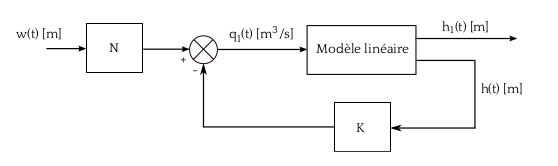
\includegraphics[scale=0.5]{fig2.png}
\captionof{figure}{\textit{ Retour d’état.}}
\label{fig2} 
\end{center}



 \chapter{Implantation De Le Loi De Commande}
      
       
 
 
\addcontentsline{toc}{chapter}{Implantation De Le Loi De Commande}
 \section{Calcul D’un Observateur Minimal Identité}

 \subsection{Le modèle linéarisé est-il observable ?}
 
 Pour voir est ce que le système étudier est observable   on va calculer la matrice de l'observabilté : \\
 Méthode analytique :\\\\
      $obs$=$\begin{bmatrix}
      C & CA & CA^{2}
      \end{bmatrix}^{T}$\\\\
      
      $obs$=$\begin{bmatrix}
      1 & 0 & 0 \\
      -0.2349 & -1.0938 & 0.9174 \\
      0.0451 & 0.2883 & -0.2717 \\
      \end{bmatrix}$
      
De même, on a vérifier avec MATLAB l'observabilité du système. \hyperref[section1.3]{(voir Annexe 3)}\label{annexe3}\\ 

 On remarque que le rang de la matrice obs est égale à la dimension du système d'ou le système est observable.
 %%%%%%%%%%%copmpleter%%%%%%%%
 
 \subsection{Calcul Du Nouveau Observateur identité }
Constitution de l'observateur minimale identité\\\\
$A$=$\begin{bmatrix}
-0.0092 & 0.0092 & 0 \\
0.0092 & -0.0198 & 0.0106\\
0 & 0.0106 & 0.0486\\
\end{bmatrix}$\\\\
Séparation de la matrice A 

$A_{11}=\begin{bmatrix}
-0.0092
\end{bmatrix}
\quad ;
A_{21}=\begin{bmatrix}
0.0092\\
0
\end{bmatrix}$\\\\


$A_{11}=\begin{bmatrix}
0.0092 & 0
\end{bmatrix}
\quad ;
A_{22}=\begin{bmatrix}
-0.0198 & 0.0106 \\
0.0106 & 0.0486
\end{bmatrix}$\\\\
 


\begin{equation}
\left\{\begin{matrix}
\dot{s}(t)=Fs(t)+(FG-GA_{11}+A_{21})y(t)+(B_{2}-GB_{1}u(t))\\
 x^(t)=s(t)+Gy(t)\\
\end{matrix}\right.
\end{equation}   
talque\\ 
$F$=$A_{22}-GA_{12}$\\\\
alors on a \\\\
$\begin{bmatrix}
f_{11} & f_{12}\\
f_{21} & f_{22}\\
\end{bmatrix}
\quad=
\begin{bmatrix}
1 & 1\\
0 & 1\\
\end{bmatrix}
\quad-
\begin{bmatrix}
g1\\
g2\\
\end{bmatrix}
\quad
\begin{bmatrix}
0.0092 & 0
\end{bmatrix}$\\\\

alors on aura \\\\
$F=
\begin{bmatrix}
f_{11} & f_{12}\\
f_{21} & f_{22}\\
\end{bmatrix}
\quad=
\begin{bmatrix}
(1-0.0092g_{1}) & 1\\
(-0.0092g_{2}) && 1\\
\end{bmatrix}$\\\\

puis en calcule  le déterminent de cette matrice puis on va faire l'identification avec le polynôme désiré\\\\

$det(\lambda I-F)= 2-0.0092g_{1}\lambda-0.0092_{g2}$\\

$P_{désiré}=(\lambda+0.11)(\lambda+0.17)\\$
           


par identification on trouve:\\\\

$G=\begin{bmatrix}
0.1393^{3}\\
3.9546^{3}\\
\end{bmatrix}
\quad
F=\begin{bmatrix}
-1.3014 & 0.0106\\
 -36.3807 & -0.0486\\
\end{bmatrix}$\\\\

$Calcule De G_{tild} et H_{tild}$:\\\\

$G_{tild}=FG-GA_{11}+A_{21}
\quad\\\\
G_{tild}=\begin{bmatrix}
-0.0904^{3}\\
 -2.5679^{3}\\
\end{bmatrix}$\\\\
$B_{11}=\begin{bmatrix}
64.9351
\end{bmatrix}
\quad 
B_{21}=\begin{bmatrix}
0\\
0
\end{bmatrix}$


$H_{tild}=B_{21}G-GB_{11}
\quad\\\\
\begin{bmatrix}
-0.0904^{5}\\
 -2.5678^{5}\\
\end{bmatrix}$\\\\

\begin{equation}
\left\{\begin{matrix}
\dot{s}(t)=\begin{bmatrix}
-1.3014 & 0.0106\\
 -36.3807 & -0.0486\\
\end{bmatrix}s(t)+(\begin{bmatrix}
-1.3014 & 0.0106\\
 -36.3807 & -0.0486\\
\end{bmatrix}\begin{bmatrix}
0.1393^{3}\\
3.9546^{3}\\
\end{bmatrix}-\begin{bmatrix}
0.1393^{3}\\
3.9546^{3}\\
\end{bmatrix}A_{11}\\
+A_{21})y(t)+(B_{2}-
\begin{bmatrix}
0.1393^{3}\\
3.9546^{3}\\
\end{bmatrix}B_{1}u(t))\\
 x^(t)=s(t)+\begin{bmatrix}
0.1393^{3}\\
3.9546^{3}\\
\end{bmatrix}y(t)\\
\end{matrix}\right.\\\\
\end{equation}   
On a aussi calculer l'observateur minimal identité avec Matlab \hyperref[section1.3]{(voir Annexe 3)}\label{annexe3}\\
 
 \subsection{Insertion Dans Notre  Schéma Simulink l’observateur sous la forme d’un bloc State-Space avec le bouclage déterminé précésemment.}

\begin{center}
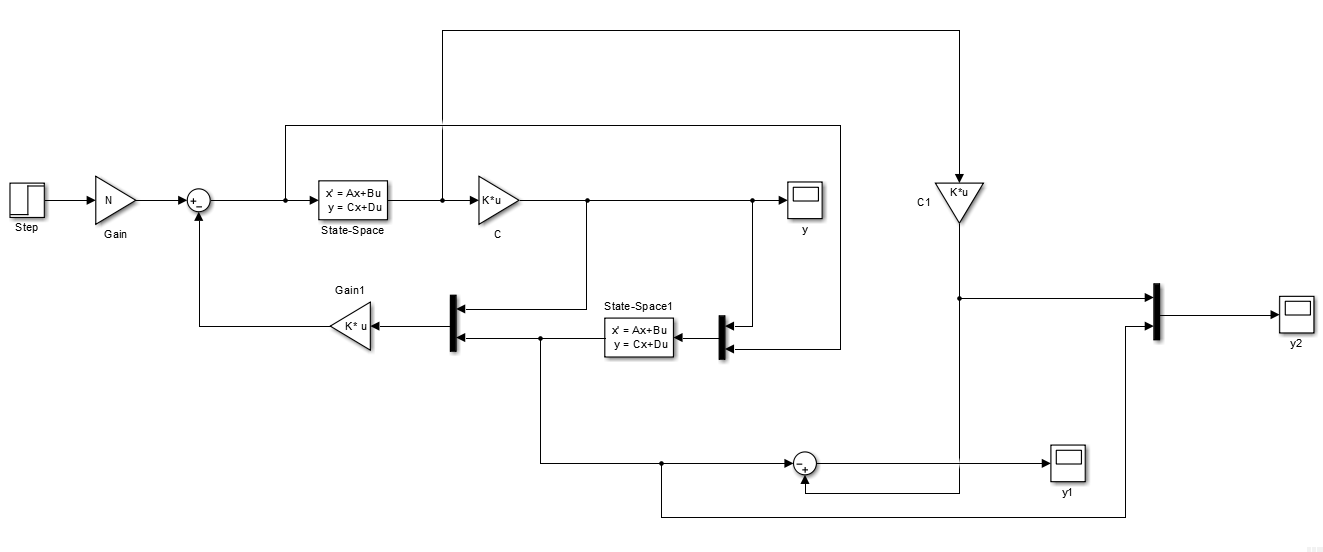
\includegraphics[scale=0.4]{schemabloc2.PNG}
\captionof{figure}{\textit{Schéma simulink avec l'observateur minimal identité.}}
\label{fig1} 
\end{center}   
  
 \subsection{Vérification, que les états estimés convergent vers les états réels du système linéarisé.\\\\} 
 
\begin{center}
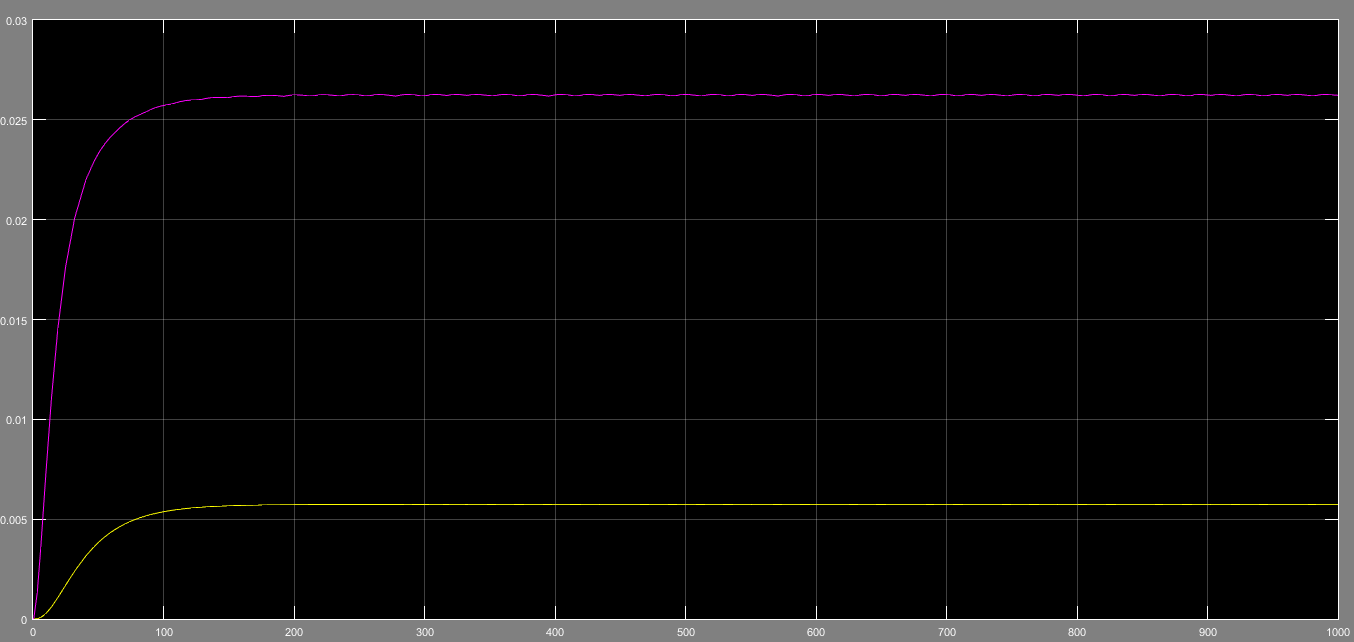
\includegraphics[scale=0.4]{Y1.PNG}
\captionof{figure}{\textit{le tracé des sorties éstimées.}}
\label{fig3} 
\end{center}
 
 Selon la figure au-dessus, on remarque que la courbe de chaque état estimé converge vers son état réel.\\\\  
 
 \subsection{Évaluation De  L’influence des Conditions Initiales.\\\\}

Après avoir changé sur l'observateur minimale construit, ses conditions initiales [0 0] vers [0.5 0.5], sur Simulink on aura le tracé des deux courbes illustrées sur la figure au-dessous :\\    

\begin{center}
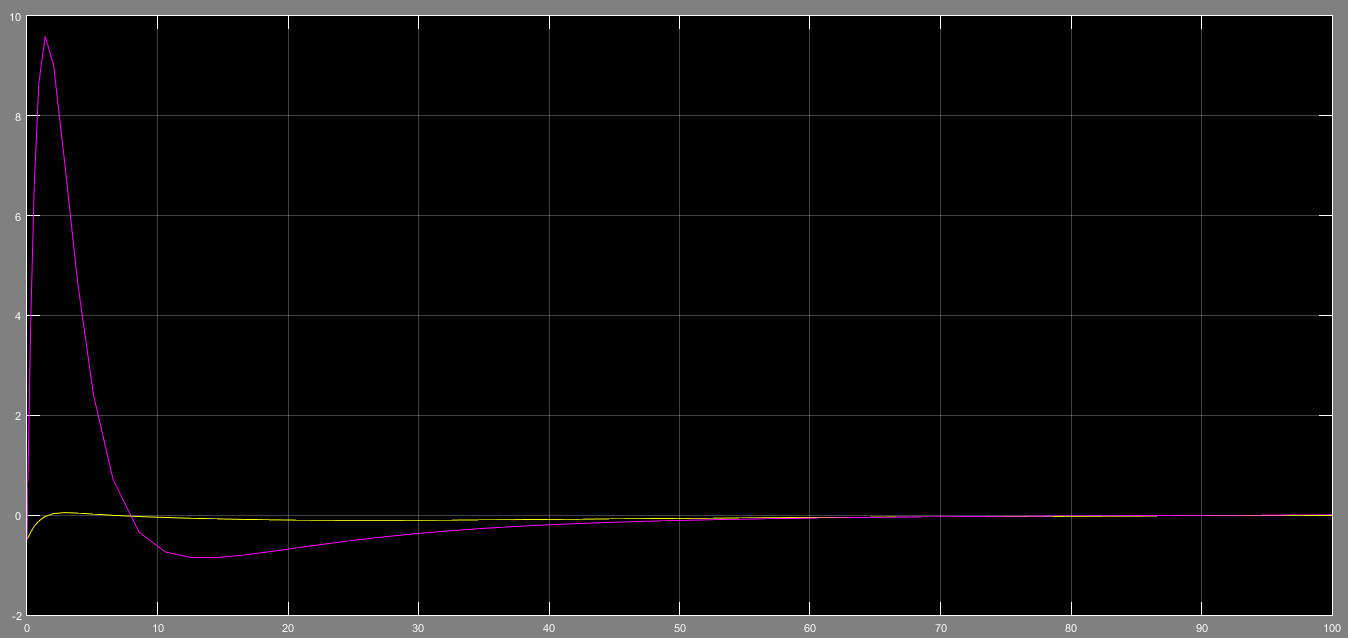
\includegraphics[scale=0.4]{Y1_condi_init.PNG}
\captionof{figure}{\textit{le tracé des sorties éstimées avce les condition initials.}}
\label{fig3} 
\end{center}

  
 \section{Bruit Sur La Sortie Mesurée\\\\}
 
 \begin{center}
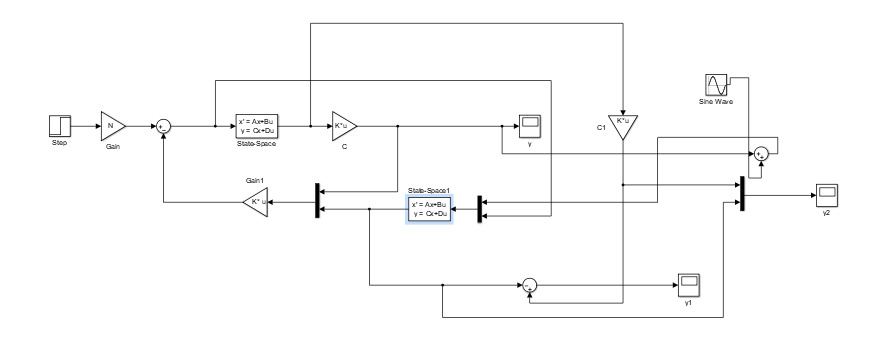
\includegraphics[scale=0.6]{schemabloc_bruit.PNG}
\captionof{figure}{\textit{schéma simulink avec l'ajout de bruit.}}
\label{fig3} 
\end{center}


\begin{center}
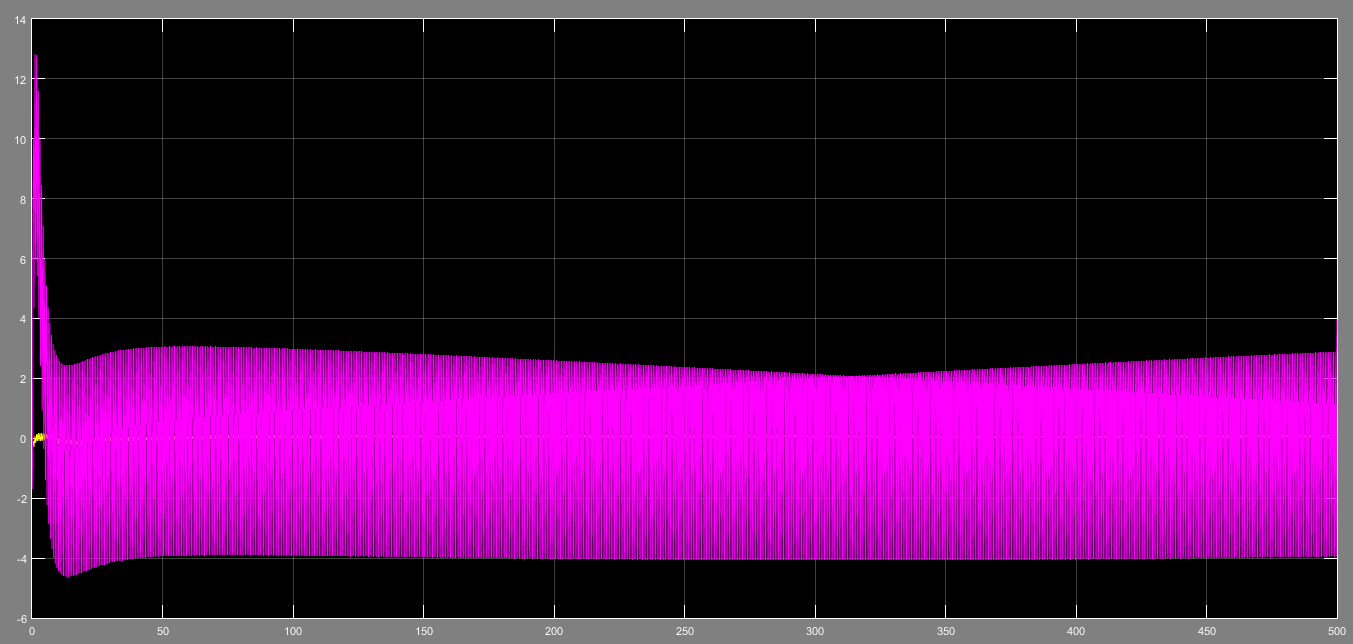
\includegraphics[scale=0.4]{Y1_bruit.PNG}
\captionof{figure}{\textit{le tracé des sorties estimées avec le bruit.}}
\label{fig3} 
\end{center}
 
 

  \subsection{Calcule d'un nouvel observateur de dynamique uniquement 2 fois plus rapide que le système bouclé par le retour d’état.\\\\}

Dans cette partie, on multiplie les deux valeurs propres $P_{2}$ et $P_{3}$ par x2, et on obtient le tracé suivant :   


\begin{center}
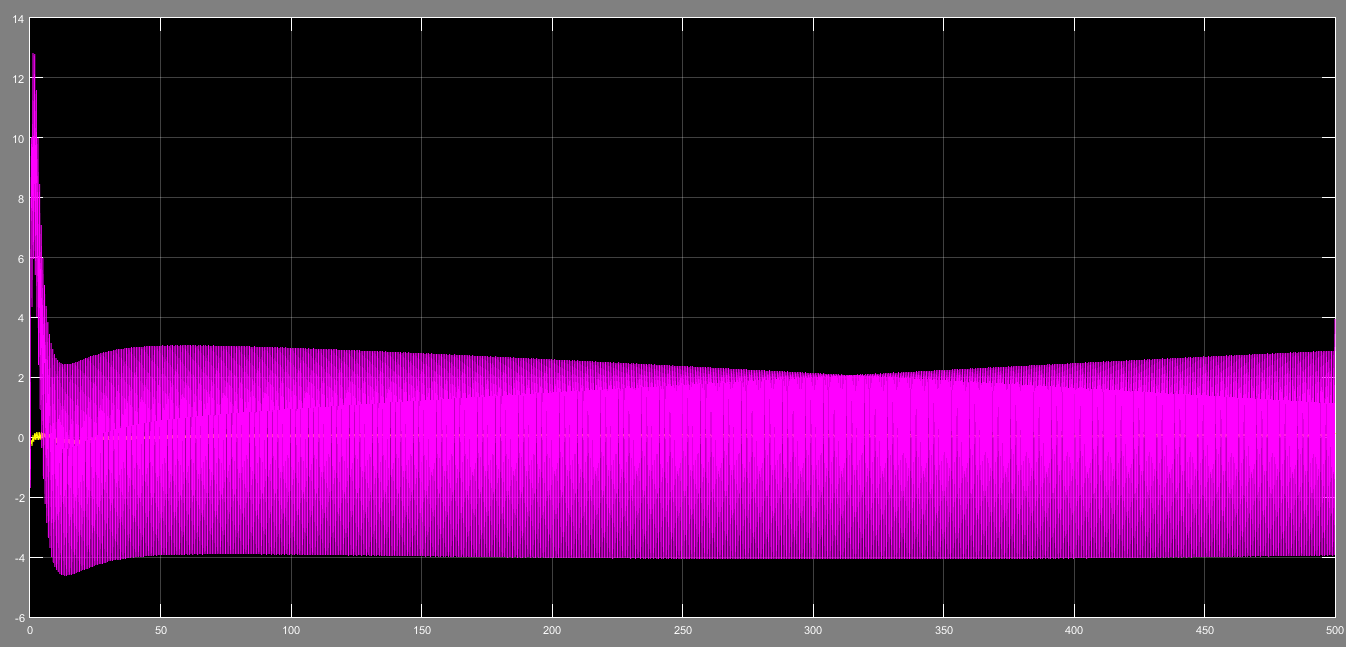
\includegraphics[scale=0.4]{Y1_2P_bruit.PNG}
\captionof{figure}{\textit{le tracé des sorties d'un nouvel observateur de dynamique 2 fois plus rapide que le système bouclé.}}
\label{fig3} 
\end{center}
  
  
  
  
  
  
  
  
  
  
 %%******************* Coclusion
\chapter*{Conclusion}
\addcontentsline{toc}{chapter}{Conclusion}
Ce TP nous a permet de prendre connaissance de la commande d'un système asservi par  retour d'état et du gain de pré-compensation, on as aussi améliorer la précision en régime établis, on aussi déterminer le lieu des pôles du système pour assurer la stabilité.




\begin{appendices}
\chapter*{Annexe 1}

\hyperref[annexe1]{(Retour)}\label{section1.1}
	
	
\begin{lstlisting}
clear all 
close all
clc

S=0.0154;
Sn=5*10^-5;
g=9.81;
H10=0.27474;
H20=0.0299;
H30=0.1368;
H00=0;
a13=0.4753*Sn*sqrt(2*g);
a32=0.4833*Sn*sqrt(2*g);
a20=0.9142*Sn*sqrt(2*g);

R13=(2*sqrt(H10-H30))/a13;
R32=(2*sqrt(H30-H20))/a32;
R20=(2*sqrt(H20-H00))/a20;

A=[-1/(S*R13) 1/(S*R13) 0;
    1/(S*R13) -(1/S)*((1/R13)+(1/R32)) 1/(S*R32);
    0 1/(S*R32) -(1/S)*((1/R32)+(1/R20))]
B=[ 1/S; 0; 0]
C=[1 0 0];
D=[0];

sys=ss(A,B,C,D);
Vp=eig(A);
Co=ctrb(sys)
rang_co=rank(Co);
%le rang=3=dimension du systeme, alors le systeme est commandable
		
			    			
	\end{lstlisting}
				
\end{appendices}





%Bibliographie 
%\bibliographystyle{alpha}
%\bibliography{biblio}




\end{document}







